\documentclass{article}

\usepackage{amsmath, amssymb}
\usepackage{graphicx, float}

\title{CGC Final Report: The Measurement of Thermal Anisotropy in Snow with Needle Probes}
\author{Joshua Holbrook}
\date{\today}

\begin{document}

\maketitle

A new method for measuring thermal conductivity is being adapted from 
the method of measuring isotropic thermal conductivity in snow with needle
probes as used by Sturm, Johnson and others, in order to enable the
determination of anisotropic thermal conductivities. This
method has particular relevance to measuring thermal conductivity of natural
snowpacks where conductivity can be strongly anisotropic due to structures that
develop from vapor transport-induced metamorphism, self-compaction and other
mechanisms, and where there are known discrepancies between density-conductivity
relations empirically derived from guarded hot plate and needle probe methods.

Both analytically-based solutions and finite element numerical solutions to the
anisotropic case are used to calculate the expected effective thermal
conductivity as a function of anisotropic thermal conductivity and needle
orientation. Additionally, preliminary measurements of both anisotropic salt/sugar
layered samples and of snow were taken. Both suggest that detecting anisotropy
in such materials is possible, though made difficult by variability between
measurements and the requirement of multiple
measurements at various angles. These studies suggest that
anisotropy in snow may be able to explain in part the discrepancies between
guarded hot plate and needle probe measurements in certain cases.

\begin{figure}[h]
\centering
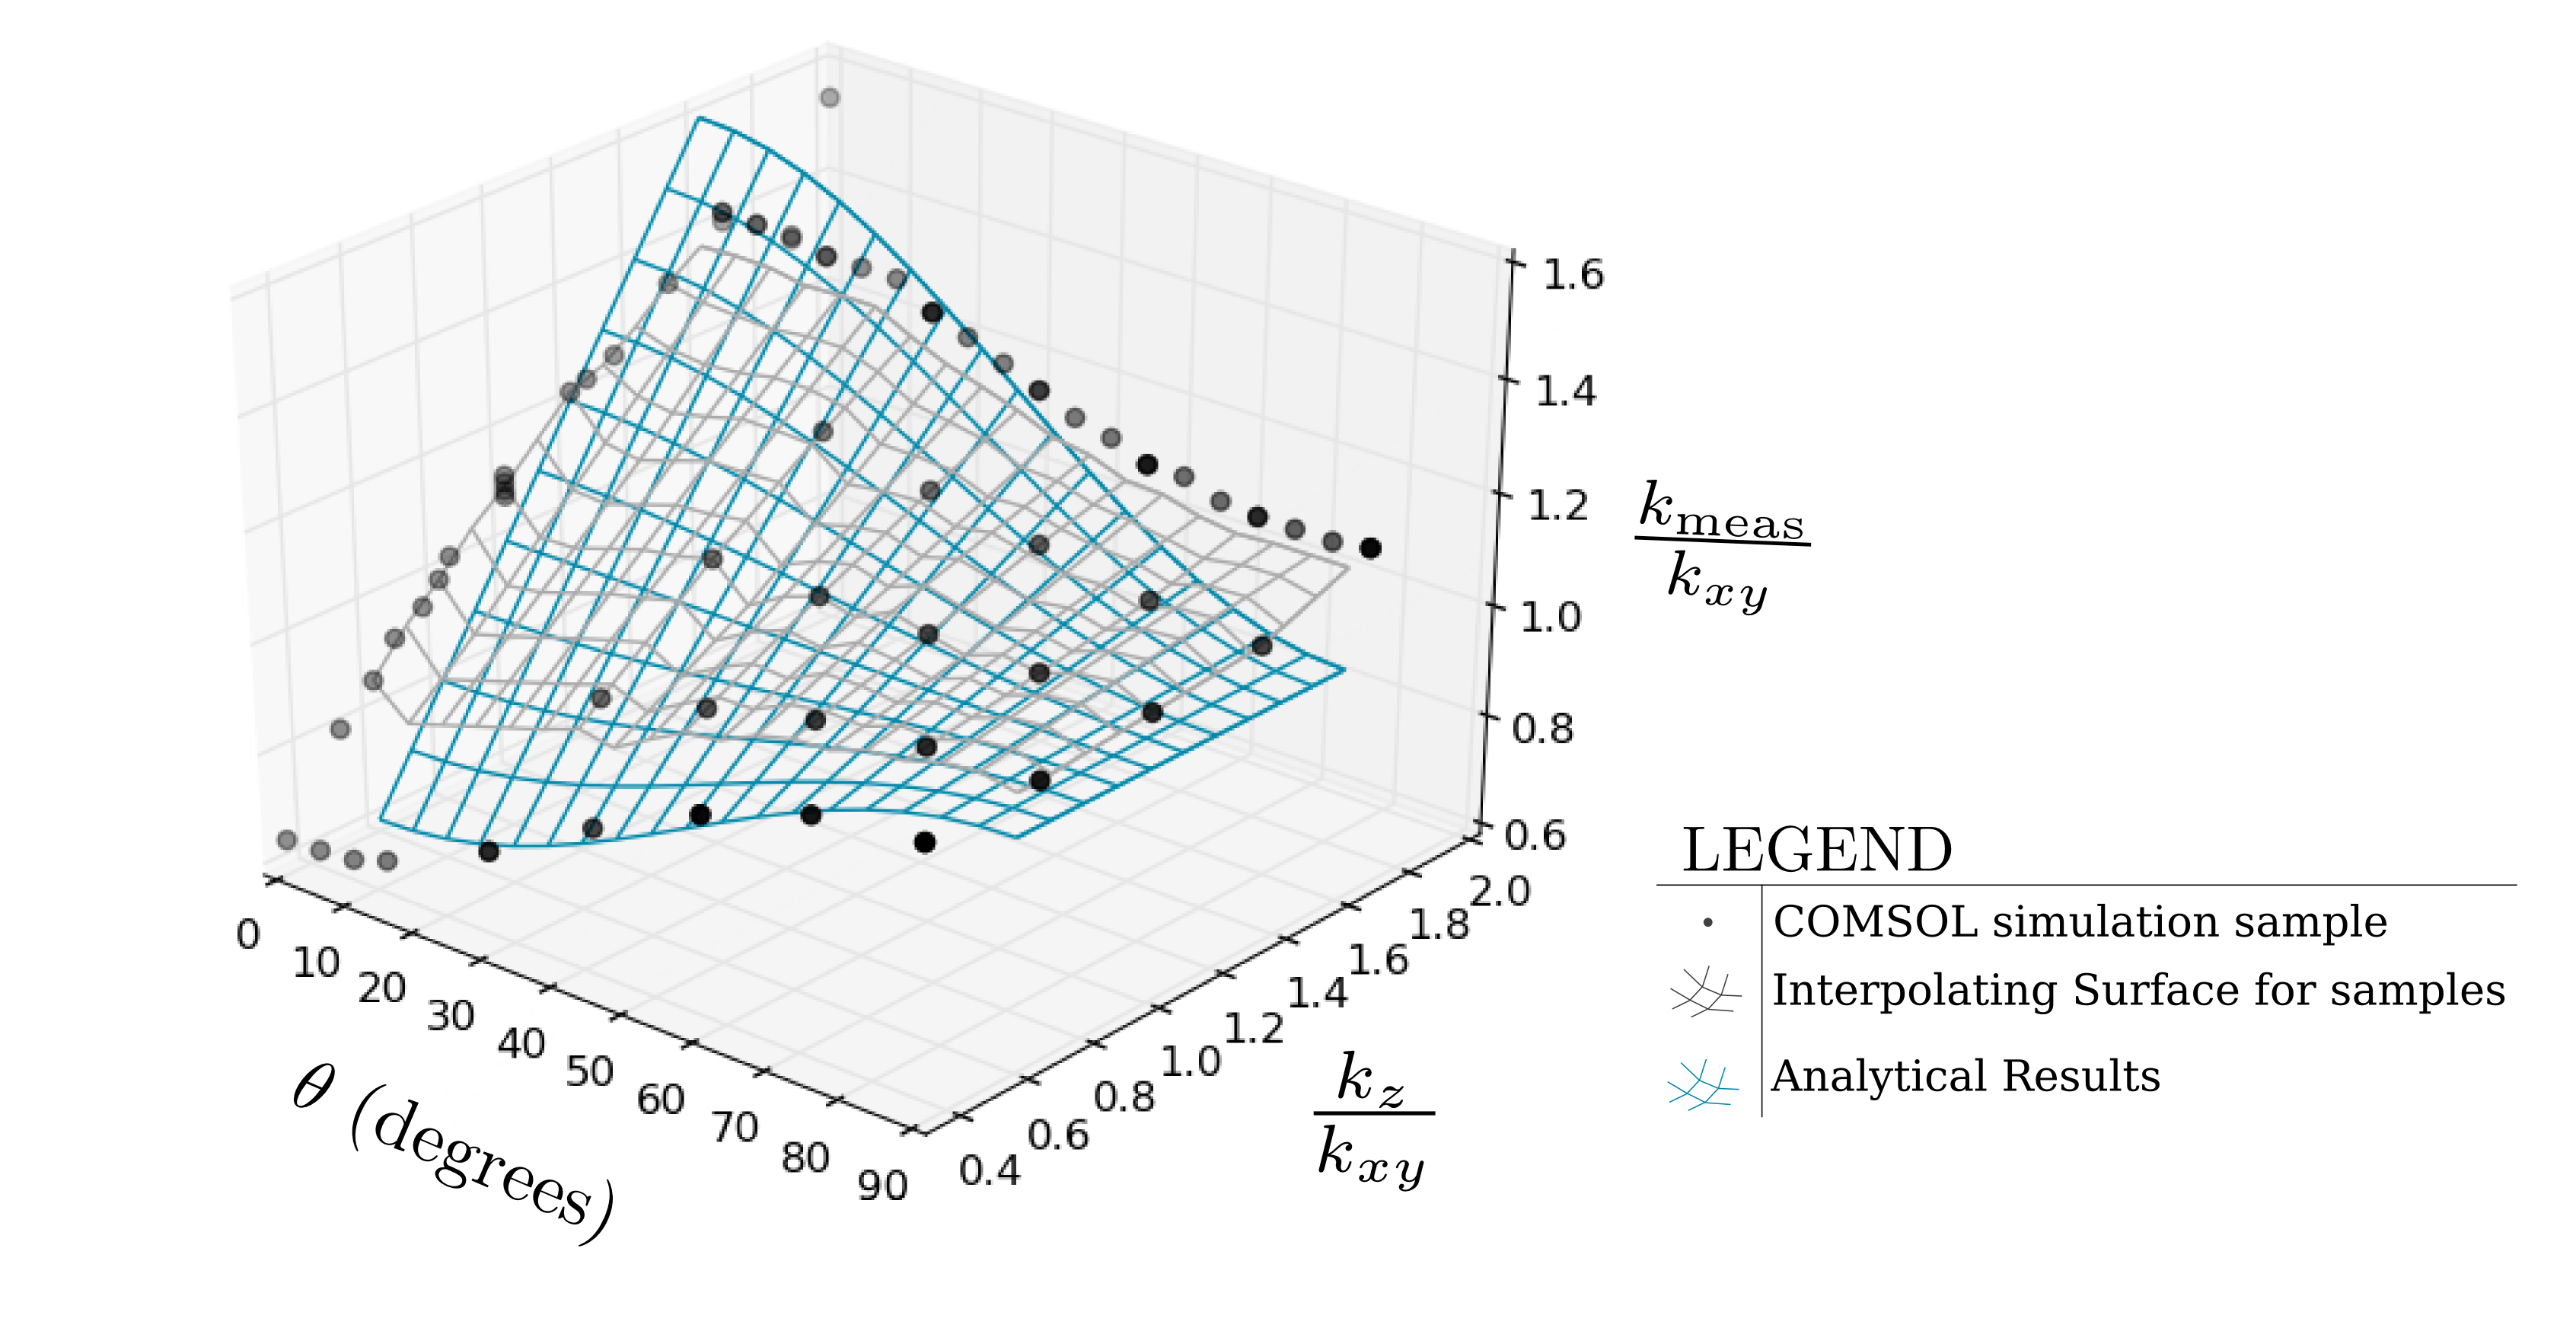
\includegraphics[width=\textwidth]{numvanal.png}
\caption{A comparison of the numerical results and the analytical theory shows
general agreement. Grey dots represent numerical simulation results, the grey surface represents an interpolating surface of the dots, and the blue surface represents the analytical model. Disagreement between the two may be due to edge effects and/or numerical
model convergence issues.}
\label{fig:numvanal}
\end{figure}


\end{document}
